\documentclass{beamer}
\setbeamercovered{transparent}
\usepackage{epstopdf}
\usepackage{listings}
\usepackage{lipsum}
\usepackage{subfig}
\usepackage{algorithm}
\usepackage{algorithmicx}
\usepackage{cite}
\usepackage{lipsum}
\usepackage{amssymb}
\usepackage{color}
\usepackage{IEEEtrantools}
\usepackage{booktabs}
\usepackage{texpower}
\usepackage{amsmath}
\usepackage{caption}
\usepackage{multirow}
\usepackage{graphicx}
\newtheorem{Key points}{Key points}
\newtheorem{Summary}{Summary}
\usepackage{dblfloatfix}
%\usepackage{adjustbox}
%\usepackage{animate}
%\usepackage{movie15}
%\usepackage{subfig}
%\newtheorem{Definition}{Definition}
%\usepackage[font={small}]{caption}
\usepackage{beamerthemeshadow}
\newcommand\Fontvi{\fontsize{5}{6.2}\selectfont}
\newcommand\Fontvia{\fontsize{6}{7.2}\selectfont}
\newcommand\Fontviaa{\fontsize{8}{7.2}\selectfont}
\usepackage{listings}
\lstset{language=C++,
                keywordstyle=\color{blue},
                stringstyle=\color{red},
                commentstyle=\color{green},
                morecomment=[l][\color{magenta}]{\#},
                numbers=left,
                escapeinside=||
}

%\captionsetup{font=scriptsize,labelfont=scriptsize}
 \usetheme{Antibes}%PaloAlto
\begin{document}
\title[Lecture 6]{Data Structures and Object Oriented Programming using C++} 
\author[]{Ahsan Ijaz}
\date{}
 \frame{\titlepage}
% \AtBeginSection[]
% {
% \begin{frame}<beamer>{Table of Contents}
% \tableofcontents[currentsection,currentsubsection, 
%     hideothersubsections, 
%     sectionstyle=show/shaded,
% ]
% \end{frame}
% }

 \section{Inheritance}
\frame{\frametitle{Inheritance}
In object-oriented language, a class can obtain the properties of another class through the mechanism of inheritance.
  \begin{itemize}
  \item<1-> In C++, inheritance is supported by class derivation.
\item<2-> A derived class inherits the properties of its base class.
  \end{itemize}
 }

\begin{frame}[fragile]
\frametitle{Vehicle}
  \begin{figure}
    \centering
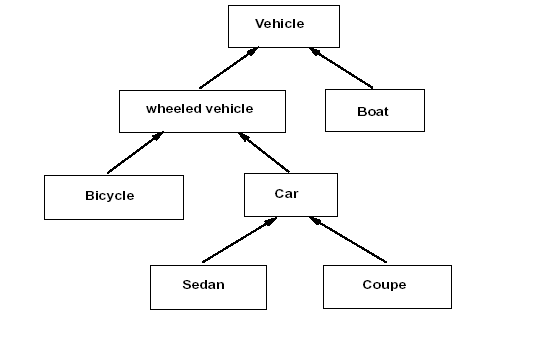
\includegraphics[width=0.8\columnwidth]{inher.png}    
\caption{Inheritance Vehicle Example}
  \end{figure}
\end{frame}

\frame{\frametitle{Inheritance}
  \begin{itemize}
\item The class that is being inherited from is called the {\color{blue}base class}. 
\item The new class is called the {\color{blue}derived class}. 
\item The set of the base and derived class instances is called the class {\color{blue}inheritance hierarchy}.
  \end{itemize}
}

\begin{frame}[fragile]
\frametitle{Inheritance}
A derived class inherits data members and member functions of its base class, and can also add its own list of generalization and specialization.
\begin{lstlisting}
class derived-class: access-specifier base-class
\end{lstlisting}
\end{frame}
\frame{\frametitle{Generalization and Specialization}
\textbf{Generalization:}
  \begin{itemize}
  \item Extend the behavior of the base class. 
  \item Add new member functions and/or data to derived class.
  \end{itemize}
\textbf{Specialization:}
\begin{itemize}
\item Modify the behavior of the base class. 
\item Change implementations in the derived class without  changing the base class interface.
\end{itemize}
}
\frame{\frametitle{Benefits of Inheritance}
Increase software reuse and quality
\begin{itemize}
\item Programmers can reuse the base classes instead of writing new classes
\item Using well-tested base classes helps reduce bugs in software.
\item Reduce code size.
\end{itemize}
Enhance software extensibility and comprehensibility
\begin{itemize}
\item Helps support more flexible and extensible architectures.
\item Useful for modeling and classifying hierarchically  related domains.
\end{itemize}
}
\begin{frame}[fragile]
\frametitle{Basic syntax of inheritance}
\Fontviaa
\begin{lstlisting}
class Pen 
{public:
	void SetLocation(int, int);
	void SetStatus(int);
private:
	int x, y, status;  
};   //end class declaration.

class ColorPen : public Pen 
{public:
	void SetColor(int);
private:
	int color;
};
\end{lstlisting}
Here Pen is the base class. ColorPen is the derived class. The keyword public indicates here the type of inheritance is public.
\end{frame}
\begin{frame}[fragile]
\frametitle{Pen inheritance}
  \begin{figure}
    \centering
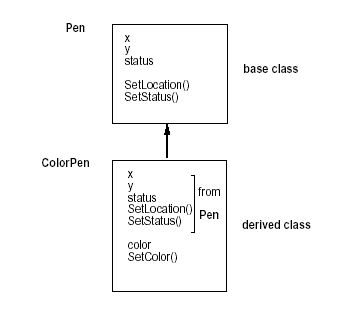
\includegraphics[width=0.6\columnwidth]{basederived.png}    
\caption{Variables of ColorPen}
  \end{figure}
\end{frame}
\frame{\frametitle{Derived Class composition}
A derived class object consists of sub-objects of its base classes and a derived class portion.
 \begin{figure}
    \centering
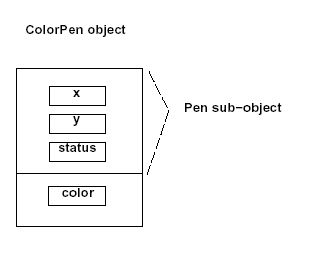
\includegraphics[width=0.6\columnwidth]{derclass.png}    
\caption{Sub-Objects}
  \end{figure}
}
\frame{\frametitle{Member Access}
\textbf{Public Member:}
  \begin{itemize}
  \item In {\color{red}public inheritance}, public members from the base class are public in its derived classes.
  \end{itemize}
\textbf{Private Member:}
\begin{itemize}
\item Private members in a base class are accessible only in the base class; they are not accessible in its derived classes.
\end{itemize}
}
\frame{\frametitle{Member access}
A derived class object consists of sub-objects of its base classes and a derived class portion.
 \begin{figure}
    \centering
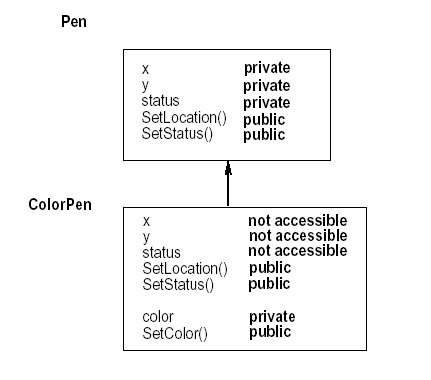
\includegraphics[width=0.5\columnwidth]{access.png}    
\caption{Member access in ColorPen}
  \end{figure}
}
\begin{frame}[fragile]
\frametitle{Member access Error}
\begin{lstlisting}
class Pen {
	public:
		void SetLocation(int, int);
		void SetStatus(int);
	private:
		int x, y, status;};
class ColorPen : public Pen {
	public:
		void SetColor(int);
		void setX(int xx){ x = xx; }//Error! 	
        private:
		int color;
};
\end{lstlisting}
\end{frame}
\frame{\frametitle{Member Access}
The private member x, y, status in class Pen can be accessed only by the implementers of class Pen.
}
\end{document}